\begin{frame}

\frametitle{Introduction: Centralized vs Distributed VCS}

\begin{multicols}{2}

\begin{figure}
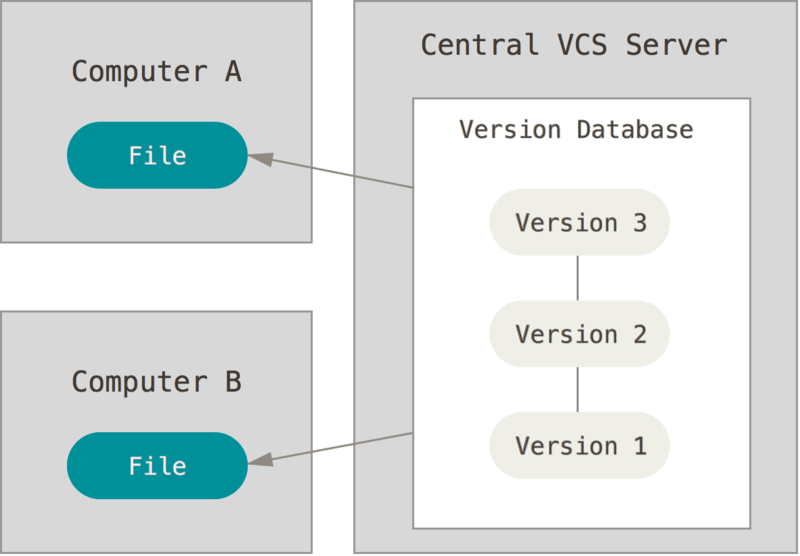
\includegraphics[scale=0.2]{centralized.png}
\caption{Centralized VCS. From \href{https://git-scm.com/book/en/v2/Getting-Started-About-Version-Control}{Git SCM}}
\label{fig:centralized}
\end{figure}

\begin{figure}
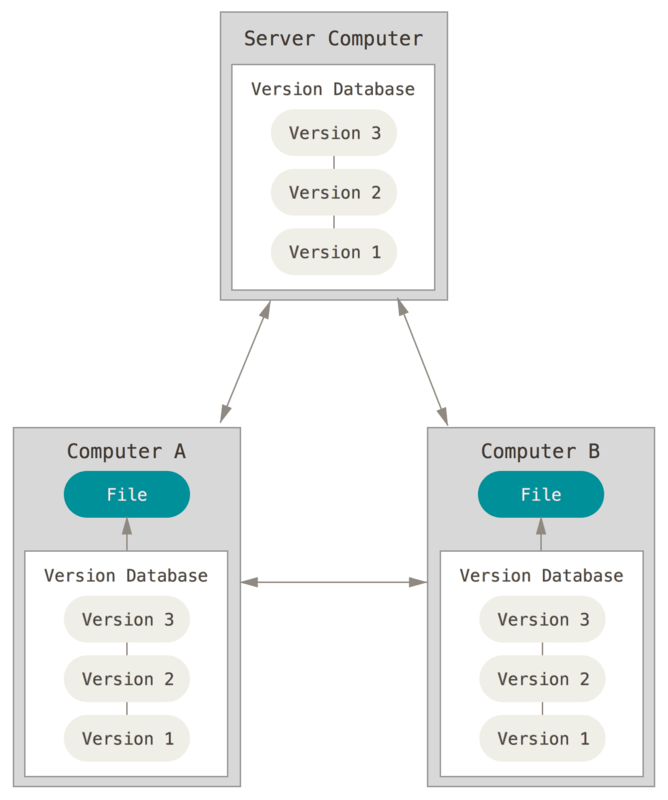
\includegraphics[scale=0.15]{distributed.png}
\caption{Distributed VCS. From \href{https://git-scm.com/book/en/v2/Getting-Started-About-Version-Control}{Git SCM}}
\label{fig:distributed}
\end{figure}

\end{multicols}

\end{frame}

\begin{frame}

\frametitle{Introduction: Centralized vs Distributed VCS}

\begin{multicols}{2}

Centralized VCS

\begin{itemize}
\item {Pros
\begin{itemize}
\item Easy administration
\item Status constantly updated
\end{itemize}
}
\item {Cons
\begin{itemize}
\item Network dependency
\item Checkouts and commits constantly
\item Branching is expensive (time)
\item Backups highly important
\end{itemize}

}
\end{itemize}


Distributed VCS

\begin{itemize}
\item {Pros
\begin{itemize}
\item No network dependency
\item More autonomy
\item Branching is easy
\item Each node have a copy of the project.
\end{itemize}
}
\item {Cons
\begin{itemize}
\item Less control of changes in server side
\item Merge conflicts are more frequent.
\end{itemize}

}
\end{itemize}

\end{multicols}

\end{frame}

\begin{frame}

\frametitle{Introduction: Centralized vs Distributed VCS}

\begin{block}{Centralized VCS}

Most popular centralized VCS are:

\begin{itemize}
\item Subversion (SVN)
\item Concurrent Versions Systems
\end{itemize}

\end{block}
\begin{block}{Distributed VCS}

Most popular distributed VCS are:

\begin{itemize}
\item \textbf{Git}
\item Mercurial
\item Bitkeeper and many more...
\end{itemize}

\end{block}
\end{frame}